\documentclass[twocolumn, 10pt]{article}
\usepackage{palatino}
\usepackage{xcolor}
\usepackage{graphicx}
\usepackage{url}
% \usepackage{graphics}
\usepackage{titling}
\setlength{\droptitle}{-1in}
\begin{document}
% \topmargin -1in
\title{Pruning Meta Learning Algorithms for Edge Computing}

\author{Lucas Tong\thanks{All authors have contributed equally} \and Daniel Ahn \footnotemark[1]}
\maketitle

\section{Introduction}
Machine Learning has had major impacts throughout all of computing but edge computing has lagged behind. Modern edge computing devices collect massive amounts of information but are unable to process it due to constraints on their computational or energy resources. Some limitations on deployment of machine learning systems on edge devices are as follows: Firstly, edge devices are frequently memory constrained. Large models are simply unable to be trained in these environments if they don't fit in the device's memory. Secondly, training models locally requires large amounts of energy and compute time. This could be detrimental to training models on battery powered edge devices such as phones or rural devices with intermittent power. Thirdly, some edge devices collect massive amounts of sensor data but are unable to upload it to cloud services due to privacy \cite{bioboios} or cellular bandwidth constraints \cite{lin2020realtime}. Ideally, models used in these circumstances are trained locally instead of on a more powerful cloud service. This is common in biotech applications \cite{bioboios} and smart agriculture \cite{farmerhicks}. 

In order to handle these challenges unique to edge computing, a possible solution comes in the form of meta learning. Meta learning is a branch of machine learning concerned with training machine learning models to adapt to new tasks quickly while taking into account previously learned tasks. These approaches are well suited to the challenges common amongst edge devices as they allow central servers to train meta models that generalize to new tasks quickly. Meta models learned through meta learning could be deployed to a fleet of small edge devices to fit to the local tasks. This alleviates many of the above problems. Meta learning allows training on edge devices which circumvents sending any information to remote servers. Fine tuning the trained meta model locally for each task specific model will be significantly faster and cost far less energy than training a new model for each new task. Meta models have the added benefit of leveraging features learned from different but related tasks to perform tasks for which there exists few data points

Amongst the many meta learning algorithms, we are currently focused on an approach known as Model Agnostic Meta Learning, MAML, outlined by Finn in \cite{finn2017modelagnostic}. MAML describes a standardized process by which meta models could be trained from any gradient descent based model in a small number of steps. We plan to explore other higher performing models in the future as well.

We intend to couple MAML with a recent development in model pruning described in \cite{frankle2019lottery}. The Lottery Ticket Hypothesis proposes a pruning algorithm that consistently uncovers sub-networks of any fully connected neural network with the same or greater test accuracy while retaining only a small fraction of the weights. Applying their sparsification algorithm to MAML has several benefits to the earlier challenges common to machine learning in edge devices. Firstly, the masked models generated from the lottery ticket hypothesis are incredibly sparse. The lottery ticket hypothesis has been shown to decrease parameter counts of networks by over 90\% with no loss in test accuracy. This could relieve memory constrained devices by storing parameters as sparse matrices. Secondly, the sparsity induced through the pruning algorithm results in significant improvements to network training time. Not only are there fewer operations to do during meta model finetuning time due to the sparse matrices but models sparsified through the process have also been shown to converge in far fewer iterations than the original dense network. Thirdly, the lottery ticket pruning process is entirely model agnostic. This synergizes well with MAML as both processes work for all networks with loss functions. Lastly, lottery ticket pruned models have been shown to generalize better than their initial unpruned dense networks. This could increase the test accuracy of our models.

\section{Related Work}

\subsection{The Lottery Ticket Hypothesis\cite{frankle2019lottery}}
The Lottery Ticket Hypothesis presents an process by which any weight based neural network could be pruned. They empirically show that networks generally contain a higher scoring sparse subnetwork. These subnetworks are discovered through an iterative train - prune - reinitialize process. Later iterations of this training process converge in a fraction of the number of training epochs. This paper is revolutionary in the field of model compression as it showed that it's possible to sparsify models without reducing their testing accuracy. 

\subsection{Drawing Early-Bird Tickets\cite{earlybird}}
The lottery ticket process is very computationally expensive but potentially unnecessary. This paper describes an alternative pruning scheme whereby winning tickets could be chosen very early in training. The early phase of network training generally consists of networks learning important patterns and they find that only the early phase is necessary for selecting pruned weights. They also suggest that winning tickets emerge under very high learning rates and low precision training. Using a different masking strategy, they propose to prune layer outputs with small batchnorm scalars instead of weights themselves. Their main contribution, however, is that they propose a novel early stopping criterion for each pruning iteration. Instead of stopping training when the validation scores drop, they generate a mask from each iteration. If the masks between several iterations are stable, they start the next pruning iteration.

\subsection{Model Agnostic Meta Learning \cite{finn2017modelagnostic}}
Model Agnostic Metal Learning provides a framework in which to train a model, known as a meta model, to be amenable to high performance when trained individually on data sets for a related but different task. The meta model is trained through a process which uses tasks as training examples. For a sampled task, the meta model undergoes a training process to become optimal for that specific task. This task specific training process is done for every task in a batch and the gradient is computed over the sum of all task specific losses and used to optimize the weights of the meta model. As this training process solely relies on gradients in the meta model and task specific model training processes, it can be applied to any gradient descent based model.

\subsection{Sparse MAML\cite{gai2019sparse}}
Sparse MAML or SMAML as presented in \cite{gai2019sparse} aims to tackle the computational complexity associated with training a meta model in the MAML framework. They accomplish this task by adding an $L_1$ regularization component to the task specific and meta model update rules. SMAML is shown to achieve performance within 2\% of MAML while only requiring 75\% of the training time. 

While sparsification can be achieved through both $L_1$ and the Lottery Ticket Hypothesis, \cite{zero_sign_supermask} shows that there can be large differences in performance between sparsity achieved through $L_1$ regularization and applying masks. For this reason we believe we are able to achieve the same, if not better, performance as SMAML with the combined Lottery Ticket MAML approach.

\begin{figure}
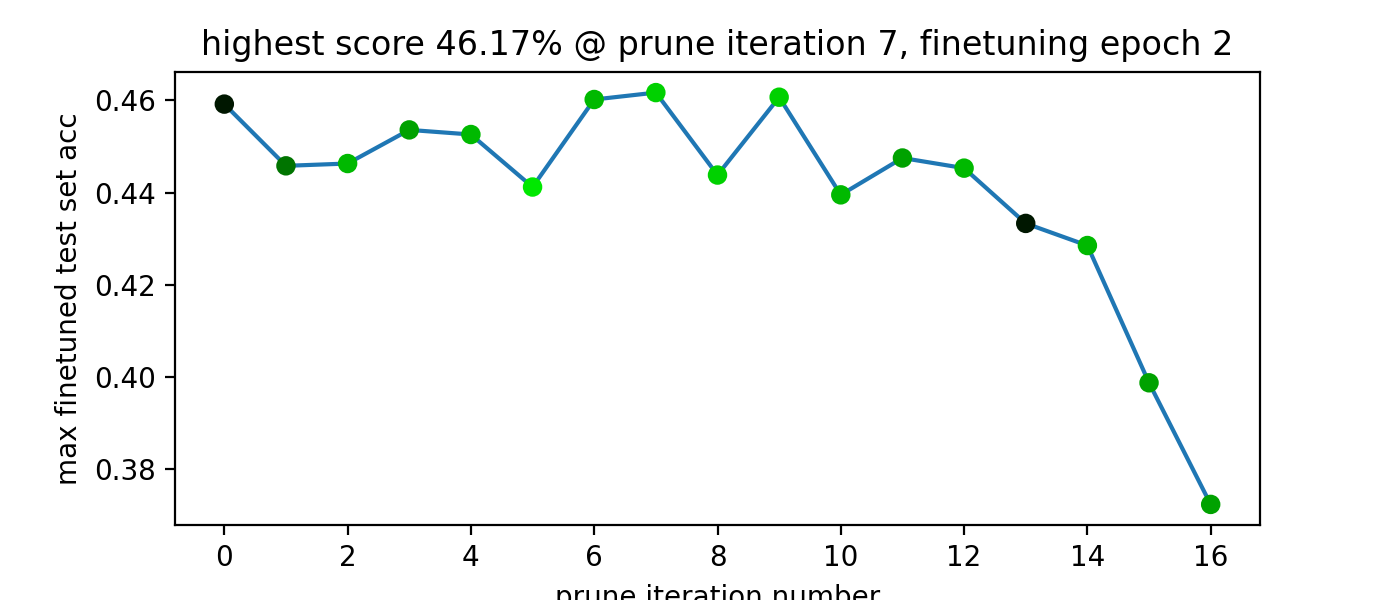
\includegraphics[scale=.4]{accs_over_time.png}
\caption{Lottery Ticket pruning applied to 4 layer convolutional meta model}
\label{lth_maml}
\end{figure}

\section{Proposed Method}
Our approach takes the sparsification afforded by the Lottery Ticket Hypothesis and applies it to the meta model. This process will allow us to determine a sparse sub meta model that should perform just as well if not better than currently used dense meta models.

The driving intuition behind this approach is the same as described in \cite{frankle2019lottery}. Removing low magnitude weights in a neural networks can improve test accuracy because it removes spurious connections that may overfit onto the training data set. By keeping a sparse meta model and allowing it to grow weights to fit specific tasks, we expect the task specific models to out perform those that were generated from dense meta models.



\section{Experimental Setup}
In order to test if sparsification of meta models can yield good test accuracy, we will be using the same data sets used in the original MAML paper. We will experiment with 5 way 1 shot and 5 way 5 shot meta learning tasks on the Mini Imagenet and Omniglot data sets.

As outlined in \cite{finn2017modelagnostic}, the meta model architecture we are using consists of a four layer VGG network. This network was chosen as it was used by both the lottery ticket hypothesis paper and the MAML paper. 

To evaluate the validity of our results, we will compare the 5 way 1 shot and 5 way 5 shot testing accuracy of our sparse meta models with figures presented in \cite{finn2017modelagnostic}. After verifying that sparse subnetworks can achieve good performance on networks trained in the MAML framework, we will move onto more sophisticated networks.

Our preliminary results are currently very promising but have only been run once. We ran into computational bottlenecks as each pruning iteration takes 3 hours on our computer (3 days to execute our experiment in total, pruning 10\% of the weights on each iteration). We were unable to tune any hyperparameters of either the lottery ticket pruning strategy or MAML and went with the paper's suggested ones. We didn't modify the learning rate scheduler and only one experiment was completed.

\begin{figure}
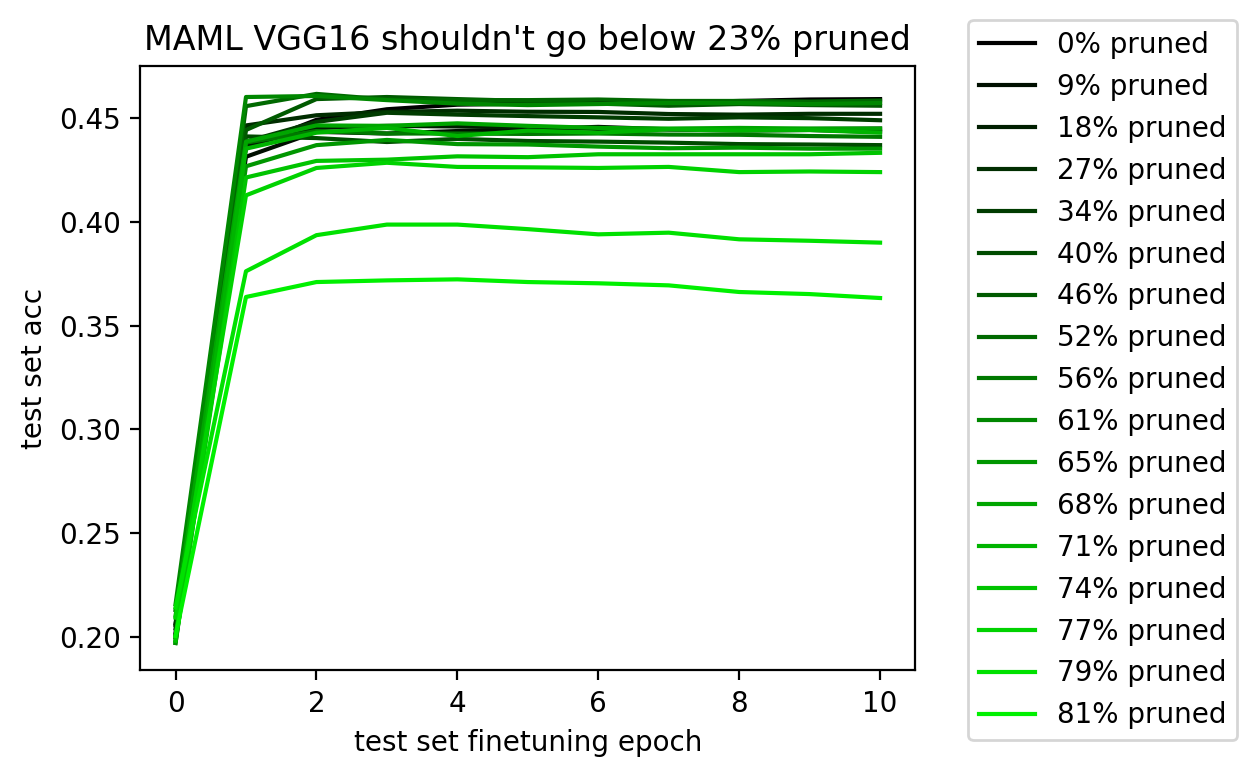
\includegraphics[scale=.4]{repeated_pruning.png}
\caption{Effects of Lottery Ticket pruning on performance of task specific model from meta model testing set}
\label{lth_vgg}
\end{figure}

\section{Preliminary Results}

Preliminary results on sparsifying the meta model can be seen in Figure \ref{lth_maml}. The graph contains maximum accuracy before early stopping triggered on 17 iterations of our lottery ticket pruned 5 way 1 shot MAML-VGG network. The shade of green of each datapoint indicates the epoch that early stopping triggered on. Lighter shades of green indicate that early stopping triggered earlier. As expected, the sparsification due to the pruning slightly increased the testing scores at prune iterations seven and nine (52\% and 61\% prune ratio respectively). The testing accuracies at this time were 46.17\% and 46.07\% and early stopping triggered on epoch 2 for both. The original network had 45.92\% testing accuracy. This indicates that our technique could significantly speed up finetuning speed as the original network trained for the maximum allotted time - 5x the finetuning time of our highest scoring pruned networks.


Figure \ref{lth_vgg} shows the same 17 training, pruning and reinitializing iterations of a MAML model. Under our current hyperparameters, we shouldn't sparsify our models below 77\% weights masked as the testing accuracy seems to drop off drastically. Later pruning iterations past iteration 17 were withheld but continued to score lower. It is possible that pruning at a lower rate for longer could allow us to compress the model past 77\%.

% weights currently aren't grown in the network during the finetuning phase.
% Increased performance by sparser subnetworks in the meta model suggest that task specific models are given the freedom to grow weights as necessary rather than repurposing already existing weights within a dense meta model.


While our scores increased with pruning, we intend to run more tests in the future. Specifically, 1) our unpruned VGG-MAML model is still scoring ~1\% lower than the original paper. 2) we set an upper bound on the number of finetuning epochs at 10 to follow the paper's precendent but the unpruned network hadn't triggered early stopping. This indicates that the unpruned network's final score could be higher than the pruned networks' scores. 3) we didn't tune any hyperparameters due to time constraints. 4) With more runs, we could be more certain that our scores aren't flukes.

\bibliographystyle{ieeetr} % We choose the "plain" reference style
\bibliography{ref} % Entries are in the "refs.bib" file

\end{document}